\documentclass[a4paper,12pt]{article}

\usepackage{ragged2e}
\justifying
\usepackage[T1]{fontenc}
\usepackage[utf8]{inputenc}
\usepackage{graphicx}
\usepackage[russian]{babel}  
\usepackage{geometry}

\geometry{total={210mm,297mm},
left=25mm,right=25mm,%
bindingoffset=0mm, top=20mm,bottom=20mm}

\usepackage{fancyhdr}
%\pagestyle{fancy}
\cfoot{Стр. \thepage}

\makeatletter
\renewcommand{\@listI}{%
\topsep=0pt }
\makeatother

\makeatletter
\let\old@itemize=\itemize
\def\itemize{\old@itemize
\setlength{\itemsep}{0pt}
\setlength{\parskip}{0pt}
\setlength{\leftskip}{0pt}
}
\makeatother

\makeatletter
\let\old@enumerate=\enumerate
\def\enumerate{\old@enumerate
\setlength{\itemsep}{0pt}
\setlength{\parskip}{0pt}
\setlength{\leftskip}{0pt}
}\makeatother

\begin{document}

\begin{titlepage}
\newpage


\begin{center}
\end{center}

\vspace{40ex}

\begin{center}
\LARGE РУКОВОДСТВО
\end{center}

\begin{center}
\Large По работе с приложением ScopeViewer
\end{center}

\vspace{55ex}

\begin{center}
\Large Санкт-Петербург
\end{center}

\begin{center}
\Large 2017
\end{center}

\end{titlepage}

\section*{\hspace{.5cm}Общие сведения }
\hspace{.5cm}Приложение ScopeViewer предназначено для отображения осциллограмм, записанных в формате COMTRADE (*.cfg) и TEXT FILE (*.txt). 

\begin{figure}[h]
\centering
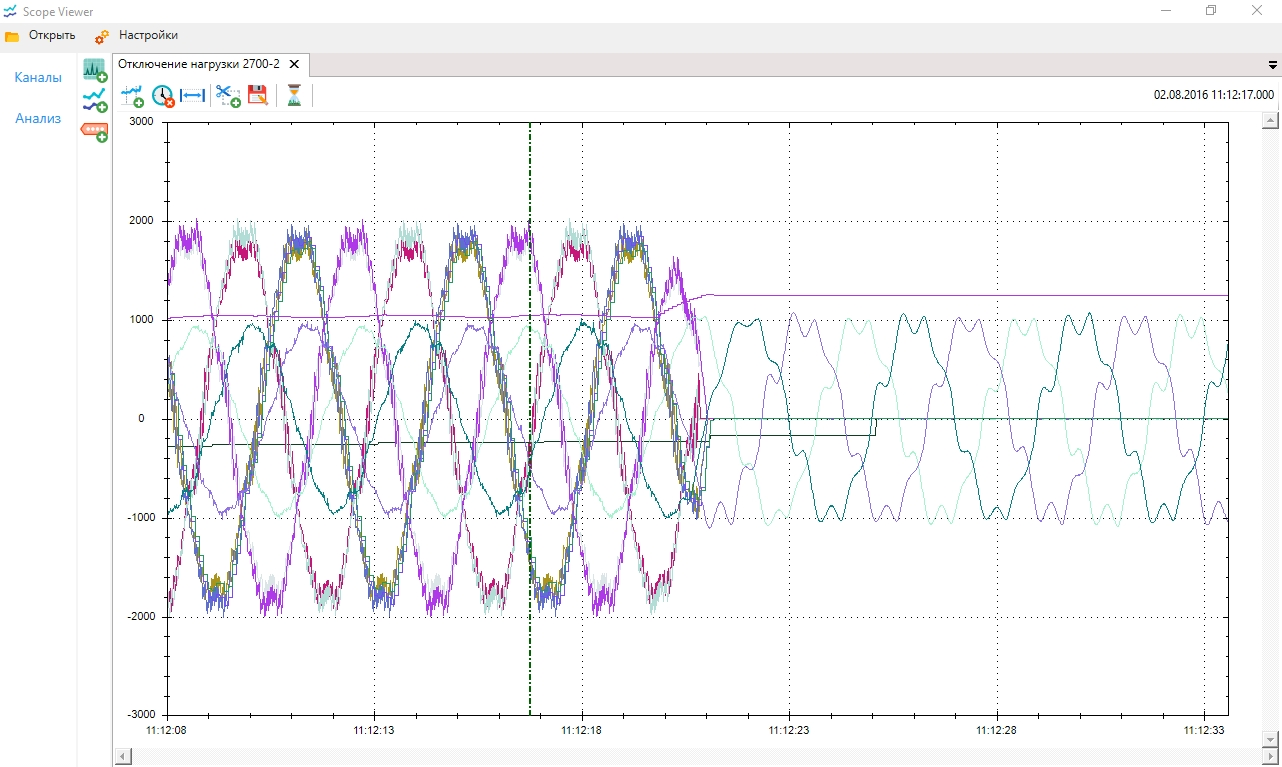
\includegraphics[width=80ex]{image/MainWindow.jpg}
\caption{Главное окно приложения.}
\end{figure}

\section*{\hspace{.5cm}Элементы управления }
\hspace{.5cm}В  верхней  части  окна  расположена  панель  инструментов,  на  которой расположены  кнопки «Открыть» и «Настройки», позволяющие открыть файл осциллограммы и настроить параметры приложения. Кнопки «Каналы» и «Анализ» дают возможность настроить параметры каналов осциллограмм и просмотреть мгновеные значения. 

\section*{\hspace{.5cm}Настройка каналов }
\hspace{.5cm}При открытие меню «Каналы» , отоброзятся настройки каналов открытых осциллограмм. Чтобы увидеть подробную информацию о канале необходимо нажать по его названию. Ниже приведены параметры, которые можно изменить в меню настройки каналов.

\begin{figure}[h]
\centering
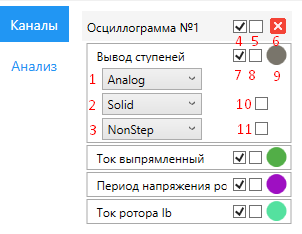
\includegraphics[width=40ex]{image/Channel.png}
\caption{Настройка каналов.}
\end{figure}

\begin{enumerate}
\item - Выбор типа канала аналоговый или цифровой. 
\item - Выбор типа линии отображаймого канала: сплошная, пунктирная, точечная.
\item - Выбор типа линии отображаймого канала.
\item - Отобразить или скрыть все каналы осциллограммы на графике.
\item - Выбрать все каналы осциллограммы.
\item - Закрыть осциллограмму.
\item - Отображение отдельного канала. 
\item - Выбрать канал.
\item - Изменить цвет линии отображения канала.
\item - Включить сглаживание.
\item - Отображать канал толстой линией.
\end {enumerate}

\section*{\hspace{.5cm} График осциллограммы}
\hspace{.5cm}Каждая открытая осциллограмма имеет собственную панель инструментов. В верхнем правом углу отображается штамп времени. Основные инструменты панели перечислены ниже.
\begin{enumerate}
\item 
\includegraphics[width=4ex]{image/Stocks_Add.png} - Добавить куросры . Для перемещения курсоров нужно нажать по нему и отпустить, после этого его можно свободно перемещать. В меню «Анализ» будут отображатся мгновенные значения каналов в положениях курсоров. 
\item 
\includegraphics[width=4ex]{image/Watch_Add.png} - Добавить штамп времени на график.
\item 
\includegraphics[width=4ex]{image/Width-48.png} - Масштабирование по горизонтали.
        
\includegraphics[width=4ex]{image/Height-48.png} - Масштабирование по вертикали. 
	  
\includegraphics[width=4ex]{image/Resize-48.png} - Масштабирование по горизонтали и вертикали.
\item 
\includegraphics[width=4ex]{image/Cutting_Add.png} - Вырезать участок осциллограммы.
	 
\includegraphics[width=4ex]{image/Cut_Apply.png} - Применить действия.
\item 
\includegraphics[width=4ex]{image/Save_as_48.png} - Сохранить осциллограмму. Осциллограмма сохраняется в формате TEXT FILE (*.txt). 
\item 
\includegraphics[width=4ex]{image/Time_abs.png} - Переключение между абсолютным и относительным временем. 
\end {enumerate}

\section*{\hspace{.5cm} Дополнительные возможности}
\hspace{.5cm} Инструмент «Добавить новый график»  
\includegraphics[width=4ex]{image/Chromatography.png}  позволяет создать новую осциллограмму. Для этого необходимио выбрать интересующие каналы в меню «Каналы». 

Инструмент «Объеденить осциллограммы»  
\includegraphics[width=4ex]{image/Line_Chart.png}  позволяет объеденить каналы различных осциллограмм в одну, при условии что они следуют друг за другом. Для этого необходимио в меню «Каналы» выбрать интересующие каналы в осциллограммах. 

Инструмент «Открыть дискретный канал»  
\includegraphics[width=4ex]{image/Dig_Add.png}  позволяет раскрыть канал по битам, при этом тип рассматриваемого канала должен быть дискретный. Одновременно можно рассматривать только один дискретный канал. При открытии будет предложено выбрать дискретность канала.

\begin{figure}[h]
\centering
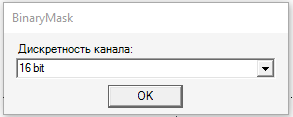
\includegraphics[width=40ex]{image/BinaryMask.png}
\caption{Дискретность канала.}
\end{figure}

\section*{\hspace{.5cm} Настройки приложения}

\end{document}
